% cjupiter-allinone-path.tex

% !TEX program = pdflatex
\documentclass{standalone}

\usepackage{tikz}
\usetikzlibrary{shapes, positioning, arrows.meta, calc, backgrounds, fit}

\def\hdist{1.8}
\def\vdist{1.8}

\newcommand{\state}[2]{% #1: state label; #2: position
  \node (#1) [circle, inner sep = 0pt, minimum size = 10mm, text width = 10mm, align = center, draw, #2, font = \Large] {$#1$};
}

\tikzset{every lower node part/.style = {red}}
\newcommand{\statesplit}[3]{% #1: state upper label; #2: state lower label; #3: position
  \node (#1) [circle split, draw, minimum size = 6mm, text width = 10mm, align = center, #3, font = \Large]
  {
	$#1$
	\nodepart{lower}
	$#2$
  };
}

\newcommand{\transition}[4][]{% #2: start state; #3: end state; #4: transition label; #1: transition label position (optional)
  \draw[>=Stealth, ->] (#2) to node [rectangle, draw, above = 2pt, sloped, #1, font = \small] {#4} (#3);
}

\newcommand{\ins}[2]{$\textsc{Ins}(#1,#2)$}
\newcommand{\del}[2]{$\textsc{Del}(#2)$} % ignore #1

\tikzset{node distance = \vdist and \hdist}
\tikzset{path/.style = {draw, rounded corners, ultra thick, #1}}

\begin{document}
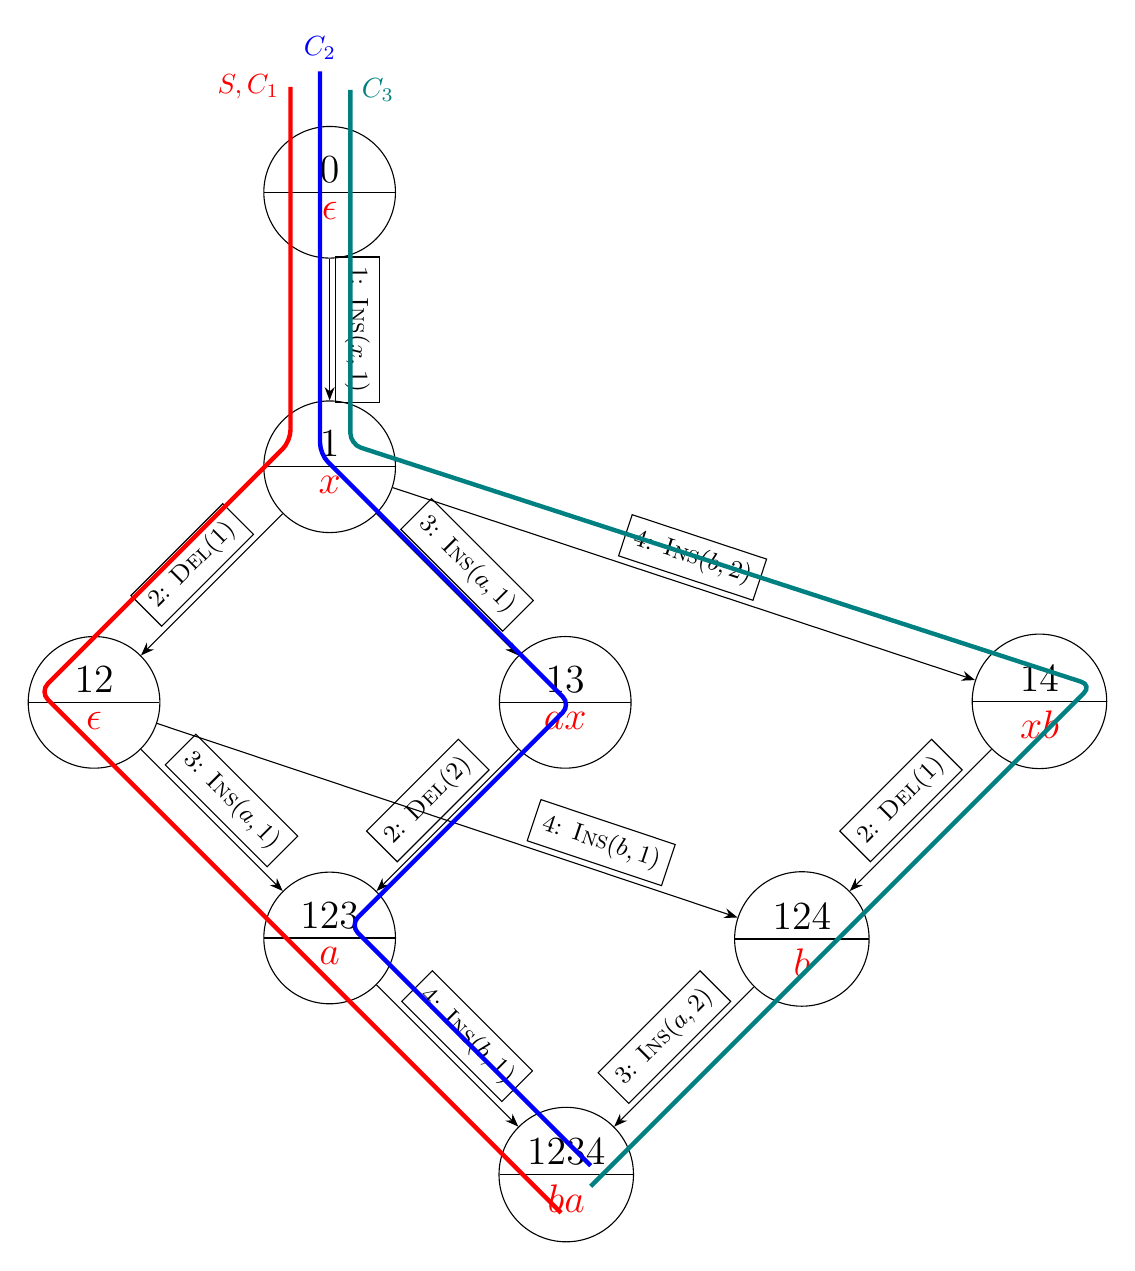
\begin{tikzpicture}
  \statesplit{0}{\epsilon}{}
  \statesplit{1}{x}{below = of 0}
  \transition{0}{1}{1: \ins{x}{1}}

  \statesplit{12}{\epsilon}{below left = of 1}
  \statesplit{13}{ax}{below right = of 1}
  \statesplit{123}{a}{below right = of 12}
  \transition{1}{12}{2: \del{x}{1}}
  \transition{1}{13}{3: \ins{a}{1}}
  \transition{12}{123}{3: \ins{a}{1}}
  \transition{13}{123}{2: \del{x}{2}}

  \statesplit{124}{b}{below right = of 13}
  \transition[near end]{12}{124}{4: \ins{b}{1}}
  
  \statesplit{1234}{ba}{below right = of 123}
  \transition{124}{1234}{3: \ins{a}{2}}
  \transition{123}{1234}{4: \ins{b}{1}}

  \statesplit{14}{xb}{above right = of 124}
  \transition{1}{14}{4: \ins{b}{2}}
  \transition{14}{124}{2: \del{x}{1}}

  \path[path = {red}] ($(0.north) + (135:20pt)$) node[left] 
  	(sc1) {$S, C_1$} -- ++(-90:2.5*\vdist) -- ++(-135:2.5*\vdist) -- ++(-45:5.2*\vdist); % -- ++(-50:2.6*\vdist);
  \path[path = {blue}] ($(0.north) + (100:20pt)$) node[above = 0pt] 
  	(c2) {$C_2$} -- ++(-90:2.7*\vdist) -- ++(-45:2.5*\vdist) -- ++(-135:2.2*\vdist) -- ++(-45:2.4*\vdist);
  \path[path = {teal}] ($(0.north) + (60:15pt)$) node[right] 
  	(c3) {$C_3$} -- ++(-90:2.5*\vdist) -- ++(-18:5.5*\vdist) -- ++(-135:5.0*\vdist);
\end{tikzpicture}
\end{document}